% This file was created by matlab2tikz.
%
\definecolor{mycolor1}{rgb}{0.12941,0.12941,0.12941}%
%
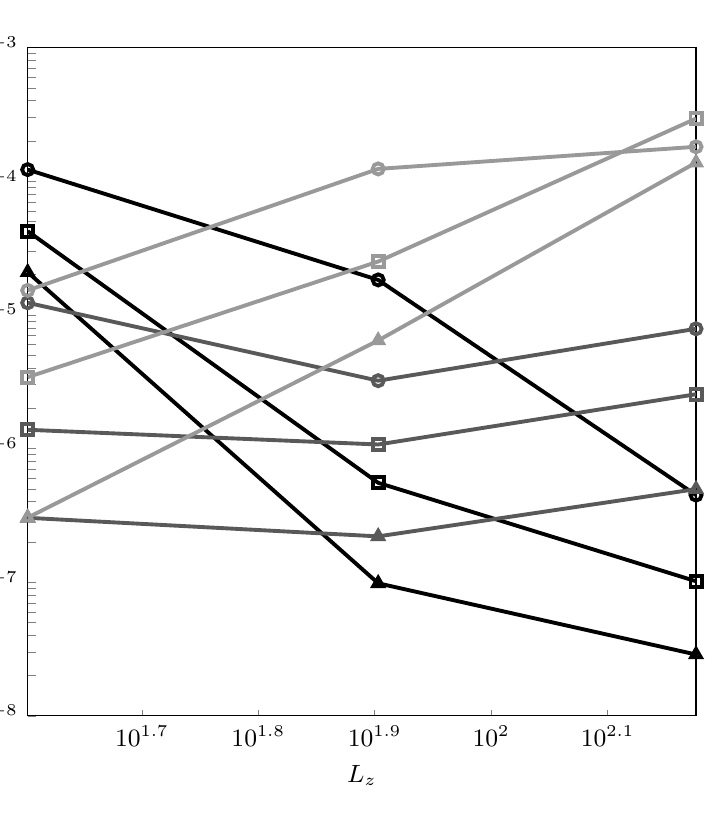
\begin{tikzpicture}[trim axis left,trim axis right]

\begin{axis}[%
width=11.252in,
height=7.131in,
at={(1.887in,0.962in)},
scale only axis,
clip=true,
xmode=log,
xmin=40,
xmax=150,
xminorticks=true,
xlabel style={font=\color{mycolor1}},
xlabel={$L_z$},
ymode=log,
ymin=1e-08,
ymax=0.001,
yminorticks=true,
ylabel style={font=\color{mycolor1}},
ylabel={$|\hat{w}|_{\partial\Omega}/\max|\hat{w}|$},
axis background/.style={fill=white},
clip=true,
clip mode=individual,
axis lines=box,
xtick pos=bottom,
ytick pos=left,
tick align=inside,
major tick length=2pt,
width=0.7\linewidth,
height=0.7\linewidth,
every axis/.append style={font=\fontsize{9}{9}\selectfont},xlabel style={font=\fontsize{9}{9}\selectfont},title style={font=\fontsize{9}{9}\selectfont},
legend style={font=\fontsize{8}{9}\selectfont,inner sep=1pt,row sep=1pt,column sep=2pt,nodes={scale=1.00},draw=none},legend image post style={xscale=0.35},
legend columns=1,
scaled x ticks=false,
tick label style={/pgf/number format/fixed,/pgf/number format/precision=2},
every x tick label/.append style={font=\fontsize{9}{9}\selectfont\color{black}},
every y tick label/.append style={font=\fontsize{9}{9}\selectfont\color{black}},
,,
colormap={sigmamap}{rgb(0.0000)=(0.0200,0.1880,0.3800); rgb(0.1000)=(0.0743,0.3456,0.5616); rgb(0.2000)=(0.1918,0.4980,0.7060); rgb(0.3000)=(0.3890,0.6708,0.8226); rgb(0.4000)=(0.7552,0.8682,0.9228); rgb(0.5000)=(0.9690,0.9689,0.9689); rgb(0.6000)=(0.9425,0.8044,0.7614); rgb(0.7000)=(0.8767,0.4910,0.4020); rgb(0.8000)=(0.7869,0.2866,0.2470); rgb(0.9000)=(0.6186,0.1239,0.1568); rgb(1.0000)=(0.4040,0.0000,0.1220)}
]
\addplot [color=black, line width=1.4pt, mark=o, mark options={solid, black}, forget plot]
  table[row sep=crcr]{%
40	0.000122082922017751\\
80	1.8264550648696e-05\\
150	4.48648862379079e-07\\
};
\addplot [color=black, line width=1.4pt, mark=square, mark options={solid, black}, forget plot]
  table[row sep=crcr]{%
40	4.2286558367524e-05\\
80	5.54140986577913e-07\\
150	1.0165940545595e-07\\
};
\addplot [color=black, line width=1.4pt, mark=triangle, mark options={solid, black}, forget plot]
  table[row sep=crcr]{%
40	2.085120628258e-05\\
80	9.81346817669049e-08\\
150	2.87734771678776e-08\\
};
\addplot [color=white!35!black, line width=1.4pt, mark=o, mark options={solid, white!35!black}, forget plot]
  table[row sep=crcr]{%
40	1.23143508727111e-05\\
80	3.21846742084817e-06\\
150	7.8698304425833e-06\\
};
\addplot [color=white!35!black, line width=1.4pt, mark=square, mark options={solid, white!35!black}, forget plot]
  table[row sep=crcr]{%
40	1.38152551912399e-06\\
80	1.07235721395277e-06\\
150	2.54877368304647e-06\\
};
\addplot [color=white!35!black, line width=1.4pt, mark=triangle, mark options={solid, white!35!black}, forget plot]
  table[row sep=crcr]{%
40	3.03259866220868e-07\\
80	2.20242511785669e-07\\
150	4.97038542330064e-07\\
};
\addplot [color=white!60!black, line width=1.4pt, mark=o, mark options={solid, white!60!black}, forget plot]
  table[row sep=crcr]{%
40	1.52513883014817e-05\\
80	0.000123616378031903\\
150	0.000180982615194387\\
};
\addplot [color=white!60!black, line width=1.4pt, mark=square, mark options={solid, white!60!black}, forget plot]
  table[row sep=crcr]{%
40	3.4193095503207e-06\\
80	2.50540817284293e-05\\
150	0.000294283534377838\\
};
\addplot [color=white!60!black, line width=1.4pt, mark=triangle, mark options={solid, white!60!black}, forget plot]
  table[row sep=crcr]{%
40	3.03900153627522e-07\\
80	6.43471146461622e-06\\
150	0.000137835424940981\\
};
\node[overlay,right, align=left, inner sep=0, font=\color{mycolor1}]
at (rel axis cs:-0.25,1.15) {$(c)$};
\end{axis}
\end{tikzpicture}%